\documentclass[11pt,a4paper]{article}

\usepackage[utf8]{inputenc}
\usepackage[T1]{fontenc}
\usepackage{lmodern}
\usepackage[margin=2.5cm]{geometry}
\usepackage{booktabs}
\usepackage{tabularx}
\usepackage{array}
\usepackage{amsmath}
\usepackage{caption}
\usepackage{float}
\usepackage{graphicx}
\usepackage[round]{natbib}
\setcitestyle{citesep={,}}
\usepackage[hidelinks]{hyperref}

\newcolumntype{L}[1]{>{\raggedright\arraybackslash}p{#1}}
\setlength{\parskip}{4pt}
\setcounter{tocdepth}{2}

\begin{document}

% ------------------------------------------------------------------
% TITLE PAGE
% ------------------------------------------------------------------

\begin{titlepage}
    \centering
    \vspace*{2cm}

    {\Large Vrije Universiteit Amsterdam\par}
    \vspace{0.4cm}

    {\large Subjectivity Mining, 2026 edition\par}
    \vspace{0.2cm}

    {\large Lecturers Isa Maks and Ilia Markov\par}

    \vspace{3.5cm}

    {\huge\bfseries Assignment 5\par}
    \vspace{0.5cm}

    {\LARGE Ensemble methods for offensive language detection\\[0.2cm] and an error analysis across domains\par}

    \vspace{3cm}

    {\Large Group 9\par}
    \vspace{0.8cm}

    {\large
    \begin{tabular}{l}
        Ines Casado Vela \\
        Martin Ranea Marina \\
        Pablos Tselioudis Garmendia \\
        Helian X. Liu \\
    \end{tabular}\par}

    \vfill

    {\large 25 October 2026\par}

\end{titlepage}

\tableofcontents
\newpage

\noindent\textit{Content warning. This report discusses and quotes offensive language.}

% ------------------------------------------------------------------
\section{Introduction}
% ------------------------------------------------------------------

Social media platforms receive far more posts than human moderators can read, so automatic systems are used to flag offensive content. These systems need to work well on new data, and that is where they often fail. A classifier trained on one dataset can lose a lot of performance on posts from another platform or annotation project \citep{swamy2019studying,fortuna2021how}. For researchers in offensive language detection this is a practical problem as much as a scientific one. Every new platform or topic can bring a new kind of domain shift.

In Assignment 4, three transformer models were fine-tuned on OLID and on HASOC and tested on the OLID test set. The models made different mistakes, and fBERT turned out to be the most stable model across domains. This raises an obvious idea. If the models make partly different mistakes, combining them could fix some of those mistakes.

This report studies that idea. The research question is whether an ensemble of BERT and its two domain-adapted variants, HateBERT and fBERT, performs better than the best individual model, both in-domain and cross-domain. The hypothesis is that it does, but only by a small margin, because all three models share the same architecture and are trained on the same data, so their errors are expected to be strongly correlated.

To answer the question, three ensemble strategies are compared. Hard majority voting combines the predicted labels and soft voting averages the predicted probabilities. Stacking goes further and trains a meta-model on out-of-fold probabilities and six simple text features. The best ensemble is then studied in detail. Pearson correlations and significance tests explain the size of the gains, and a quantitative and a manual error analysis show which tweets remain hard.

The outcome in short. Stacking and soft voting both beat the best single model, by about one macro-F1 point in-domain and by half a point or less cross-domain. Only the in-domain gain of stacking is statistically significant. The base models are highly correlated, which limits what any ensemble can gain. Most remaining cross-domain errors are offensive tweets without any swear word, often attacks on a whole political group, and about a quarter involve a questionable gold label.

Section~\ref{sec:related} discusses related work. Sections~\ref{sec:data} and~\ref{sec:setup} briefly describe the data and the experimental setup, which are the same as in Assignment 4. Section~\ref{sec:methods} explains the base models and the three ensembles. Section~\ref{sec:results} gives the results, Section~\ref{sec:analysis} the quantitative and qualitative analysis, and Section~\ref{sec:conclusion} concludes with a discussion and ideas for future work.

% ------------------------------------------------------------------
\section{Related work}
\label{sec:related}
% ------------------------------------------------------------------

\subsection{Offensive language detection}

Offensive language detection became a standard NLP task through shared tasks such as OffensEval 2019, which introduced the OLID dataset \citep{zampieri2019olid,zampieri2019semeval}, and HASOC 2019 \citep{mandl2019hasoc}. Since then, fine-tuned transformers have dominated. The best system for OffensEval 2019 Subtask A was a fine-tuned BERT model \citep{liu2019nuli}. Later work adapted BERT to abusive language before fine-tuning. HateBERT continues pre-training on banned Reddit communities \citep{caselli2021hatebert}, and fBERT on more than a million offensive tweets from SOLID \citep{sarkar2021fbert,rosenthal2021solid}. These are the three models combined in this report.

The weak spot of these models is generalisation. Models trained on one dataset often perform much worse on another \citep{swamy2019studying,fortuna2021how}, partly because datasets are collected and labelled in different ways \citep{wiegand2019detection}. Studies on cross-domain hate speech detection found that models depend heavily on topic words and produce many false positives on new data \citep{markov2021exploring,markov2021improving}. Assignment 4 showed the same pattern for OLID and HASOC.

\subsection{Ensemble methods}

Ensembles combine several classifiers in the hope that their errors cancel out. \citet{dietterich2000ensemble} explains why this works. An ensemble only helps if its members are accurate and also make different errors, a property usually called diversity \citep{kuncheva2003measures}. Majority voting is the simplest combination rule. Stacking, introduced by \citet{wolpert1992stacked}, instead trains a meta-model on the predictions of the base models. To avoid overfitting, these training predictions must come from models that did not see the same examples, which is why stacking uses k-fold cross-validation.

Ensembles are common in offensive language shared tasks. Many of the top teams in OffensEval 2020 combined several transformer models \citep{zampieri2020semeval}, and \citet{risch2020bagging} showed that an ensemble of BERT models trained on different subsets of the data is more stable than a single model. The most direct inspiration for this report is \citet{vanaken2018challenges}. They built an ensemble of neural and classical models for toxic comment classification, which outperformed every single model, and then carried out a detailed error analysis. Their error categories, such as toxicity without swear words, sarcasm, rhetorical questions and doubtful labels, are used as the starting point for the qualitative analysis here.

\subsection{How this work differs}

Most ensemble studies in this field focus on a single dataset and report only whether the ensemble wins. This report compares three ensemble strategies on the same set of base models, in both an in-domain and a cross-domain setting. It also checks directly how correlated the base models are, which explains why the gains are small. The base models are also less diverse than in most earlier work, because they are three variants of the same BERT architecture. This makes the results relevant for anyone who plans to combine several fine-tuned BERT models, which is a very common setup in practice.

% ------------------------------------------------------------------
\section{Data}
\label{sec:data}
% ------------------------------------------------------------------

The data is the same as in Assignment 4. OLID \citep{zampieri2019olid} contains English tweets labelled as offensive or not, collected with mostly political keywords and annotated by crowd workers. HASOC \citep{mandl2019hasoc} contains English Twitter and Facebook posts, labelled as hateful or offensive, which includes profanity, versus neither. In both, label 1 means offensive and label 0 means non-offensive. Table~\ref{tab:data} shows the main statistics.

\begin{table}[H]
\centering
\caption{Statistics of the three datasets, as in Assignment 4. Mean length is in words, split on whitespace.}
\label{tab:data}
\begin{tabular}{lrrrrr}
\toprule
Dataset & Messages & Non-offensive & Offensive & Offensive \% & Mean length \\
\midrule
OLID train small & 5,852 & 3,591 & 2,261 & 38.6 & 22.4 \\
HASOC train      & 5,852 & 3,591 & 2,261 & 38.6 & 23.3 \\
OLID test        & 860   & 620   & 240   & 27.9 & 24.4 \\
\bottomrule
\end{tabular}
\end{table}

The two training sets have the same size and label balance, so neither has an advantage in amount of data. They do differ in other ways. HASOC is about events from 2019, like the Cricket World Cup and a doctors' strike in India, while OLID is mostly about American politics in 2018. HASOC also keeps real user names and uses many more hashtags. Finally, 27.4 percent of the non-offensive HASOC posts contain a swear word, against only 2.8 percent in OLID, so the two datasets do not agree on how to label swearing.

% ------------------------------------------------------------------
\section{Experimental setup}
\label{sec:setup}
% ------------------------------------------------------------------

The setup is also the same as in Assignment 4. In the \textbf{in-domain} setting, the models are trained on OLID train small and tested on the OLID test set. In the \textbf{cross-domain} setting, they are trained on HASOC and tested on the same OLID test set. The test set never changes, so any difference between the settings comes from the training data.

All systems are evaluated with the shared evaluation function from Assignment 4. It reports accuracy, macro-averaged precision, recall and F1, the same scores per class, and the confusion matrix. Macro-F1 is the main metric because only 28 percent of the test tweets are offensive. Differences between two systems on the same test tweets are tested with an exact McNemar test \citep{mcnemar1947note}. No system uses the test set for training or tuning.

% ------------------------------------------------------------------
\section{Methods}
\label{sec:methods}
% ------------------------------------------------------------------

\subsection{Overview}

Three base models are combined with three ensemble strategies. Hard voting only needs the predicted label of each base model. Soft voting needs the predicted probability of the offensive class. Stacking needs probabilities for the training data as well, and these have to be out-of-fold, so new models had to be trained for it. Table~\ref{tab:methods} summarises what each strategy uses.

\begin{table}[H]
\centering
\caption{The three ensemble strategies and what they need from the base models.}
\label{tab:methods}
\begin{tabular}{L{2.3cm}L{4.0cm}L{3.6cm}L{4.0cm}}
\toprule
Strategy & Input from base models & Extra training & Decision rule \\
\midrule
Hard voting & Predicted labels on the test set & None & Label chosen by at least two of the three models \\
Soft voting & Offensive probability on the test set & None & Mean probability at least 0.5 \\
Stacking & Out-of-fold probabilities on the training set, plus test probabilities & Three fold models per base model, and a meta-model & Logistic Regression on three probabilities and six text features \\
\bottomrule
\end{tabular}
\end{table}

\subsection{Base models}

The base models are BERT \citep{devlin2019bert}, HateBERT \citep{caselli2021hatebert} and fBERT \citep{sarkar2021fbert}. All three are BERT base models with 12 layers. HateBERT was pre-trained further on Reddit posts from communities banned for abuse, and fBERT on offensive tweets from SOLID, a large dataset built with the OLID labelling scheme. Each model is fine-tuned for binary classification with the Simple Transformers library \citep{rajapakse2019simpletransformers}. The offensive probability is the softmax of the two output scores.

Logistic Regression from Assignment 4 was left out. Its cross-domain macro-F1 of 0.51 was far below the transformers, so in a vote it would mostly add noise.

During integration a problem became clear. The three ensembles were first built by different group members, and not all of them used the same base models. The hard voting block used the BERT predictions from Assignment 4, while the soft voting block retrained BERT to get probabilities. These two BERT runs disagree on 76 test tweets in-domain and on 132 cross-domain. Stacking also needed new models, since no out-of-fold predictions existed. To compare the ensemble strategies fairly, all three were finally computed on one shared set of base models, called the \textbf{matched pool}. This pool uses the uncased BERT base model, the HateBERT models from Assignment 4 and a new fBERT model. Every new model was trained with the same settings as HateBERT in Assignment 4, which are 3 epochs, a learning rate of 2e-5, weight decay of 0.01, an effective batch size of 16, a maximum length of 128 tokens and seed 42. The original results of each block are still reported in Section~\ref{sec:original}.

\subsection{Hard majority voting}

Hard voting takes the label that at least two of the three models predict. With three voters there are no ties. Every model gets the same weight, and no training is needed. The downside is that a confident model can be outvoted by two less confident ones.

\subsection{Soft majority voting}

Soft voting averages the predicted probabilities of the offensive class and predicts offensive when the average is at least 0.5.

\begin{equation}
P_{\mathrm{soft}}(1 \mid x) = \frac{P_{\mathrm{BERT}}(1 \mid x) + P_{\mathrm{HateBERT}}(1 \mid x) + P_{\mathrm{fBERT}}(1 \mid x)}{3}
\end{equation}

Unlike hard voting, a very confident model can outweigh two models that are only slightly unsure. The weights are still equal and fixed.

\subsection{Stacking}

Stacking learns how to combine the base models \citep{wolpert1992stacked}. The meta-model needs training data that looks like test data, which means base model predictions on examples the base models did not see. To get these, each training set was split into three folds with stratified group k-fold cross-validation. Identical texts were kept in the same fold, because both training sets contain duplicates, 8 rows in OLID train small and 78 in HASOC. For each base model, three new copies were trained, each on two folds, and each predicted the third fold. This gives one out-of-fold probability per training tweet and per model, and it needed eighteen extra training runs in total.

The meta-model gets nine features per tweet. Three are the base model probabilities. The other six are simple text features. These are the log of the number of characters and of the number of words, the share of capital letters, and the number of exclamation marks and of question marks. The last one is the number of hashtags. These features were added because the assignment asks for extra features and because Assignment 4 showed that length and hashtags differ between the datasets.

The meta-model is a Logistic Regression from scikit-learn \citep{pedregosa2011scikit}, with standardised features, L2 regularisation with C = 1 and no class weights. A separate meta-model is trained for each setting, on the 5,852 out-of-fold training rows. At test time, base models trained on the full training set produce the three probabilities. The decision threshold stays at 0.5. As a check, a second stacking model with only the three probabilities was also trained.

\subsection{Analysis methods}

To explain the results, Pearson correlations between the three base models are computed in three ways, on the predicted probabilities, on the predicted labels and on error indicators, where 1 means the model is wrong on that tweet. The last one matters most for ensembles, since they can only fix errors that the models do not share.

For the quantitative error analysis, the errors of the best ensemble are counted by class, by message length and by the presence of swear words, using the same short swear word list as in Assignment 4. For the qualitative analysis, all 39 false positives and 89 false negatives of the best ensemble in the cross-domain setting were read and each was given one main error category. The categories follow \citet{vanaken2018challenges}, adapted to this data.

% ------------------------------------------------------------------
\section{Results}
\label{sec:results}
% ------------------------------------------------------------------

\subsection{Matched pool}

Table~\ref{tab:main} shows the macro-averaged scores on the matched pool, and Figure~\ref{fig:macro} compares their macro-F1.

\begin{table}[H]
\centering
\caption{Accuracy and macro-averaged scores on the OLID test set, 860 tweets, with the same three base models for every ensemble. The best score per setting is in bold.}
\label{tab:main}
\begin{tabular}{llrrrr}
\toprule
System & Setting & Accuracy & Macro-P & Macro-R & Macro-F1 \\
\midrule
BERT        & In-domain & 0.8384 & 0.8002 & 0.7947 & 0.7973 \\
HateBERT    & In-domain & 0.8407 & 0.8022 & 0.8014 & 0.8018 \\
fBERT       & In-domain & 0.8488 & 0.8136 & 0.8071 & 0.8102 \\
Hard voting & In-domain & 0.8465 & 0.8103 & 0.8054 & 0.8078 \\
Soft voting & In-domain & \textbf{0.8593} & \textbf{0.8276} & \textbf{0.8181} & \textbf{0.8226} \\
Stacking    & In-domain & 0.8558 & 0.8234 & 0.8132 & 0.8180 \\
\midrule
BERT        & Cross-domain & 0.8058 & 0.7648 & 0.7274 & 0.7415 \\
HateBERT    & Cross-domain & 0.8035 & 0.7560 & 0.7513 & 0.7536 \\
fBERT       & Cross-domain & 0.8430 & 0.8119 & \textbf{0.7851} & 0.7966 \\
Hard voting & Cross-domain & 0.8349 & 0.8029 & 0.7706 & 0.7838 \\
Soft voting & Cross-domain & 0.8465 & 0.8198 & 0.7837 & 0.7984 \\
Stacking    & Cross-domain & \textbf{0.8512} & \textbf{0.8310} & 0.7831 & \textbf{0.8016} \\
\bottomrule
\end{tabular}
\end{table}

\begin{table}[H]
\centering
\caption{Precision, recall and F1 per class on the matched pool. Class 0 is non-offensive, 620 tweets. Class 1 is offensive, 240 tweets.}
\label{tab:perclass}
\begin{tabular}{llrrrrrr}
\toprule
 & & \multicolumn{3}{c}{Class 0, non-offensive} & \multicolumn{3}{c}{Class 1, offensive} \\
\cmidrule(lr){3-5}\cmidrule(lr){6-8}
System & Setting & P & R & F1 & P & R & F1 \\
\midrule
BERT        & In-domain & 0.8836 & 0.8935 & 0.8885 & 0.7167 & 0.6958 & 0.7061 \\
HateBERT    & In-domain & 0.8889 & 0.8903 & 0.8896 & 0.7155 & 0.7125 & 0.7140 \\
fBERT       & In-domain & 0.8901 & 0.9016 & 0.8958 & 0.7371 & 0.7125 & 0.7246 \\
Hard voting & In-domain & 0.8898 & 0.8984 & 0.8941 & 0.7308 & 0.7125 & 0.7215 \\
Soft voting & In-domain & 0.8954 & 0.9113 & 0.9033 & 0.7598 & 0.7250 & 0.7420 \\
Stacking    & In-domain & 0.8924 & 0.9097 & 0.9010 & 0.7544 & 0.7167 & 0.7350 \\
\midrule
BERT        & Cross-domain & 0.8386 & 0.9048 & 0.8704 & 0.6911 & 0.5500 & 0.6125 \\
HateBERT    & Cross-domain & 0.8596 & 0.8694 & 0.8645 & 0.6524 & 0.6333 & 0.6427 \\
fBERT       & Cross-domain & 0.8725 & 0.9161 & 0.8938 & 0.7512 & 0.6542 & 0.6993 \\
Hard voting & Cross-domain & 0.8632 & 0.9161 & 0.8889 & 0.7426 & 0.6250 & 0.6787 \\
Soft voting & Cross-domain & 0.8697 & 0.9258 & 0.8969 & 0.7700 & 0.6417 & 0.7000 \\
Stacking    & Cross-domain & 0.8672 & 0.9371 & 0.9008 & 0.7947 & 0.6292 & 0.7023 \\
\bottomrule
\end{tabular}
\end{table}

\begin{figure}[H]
\centering
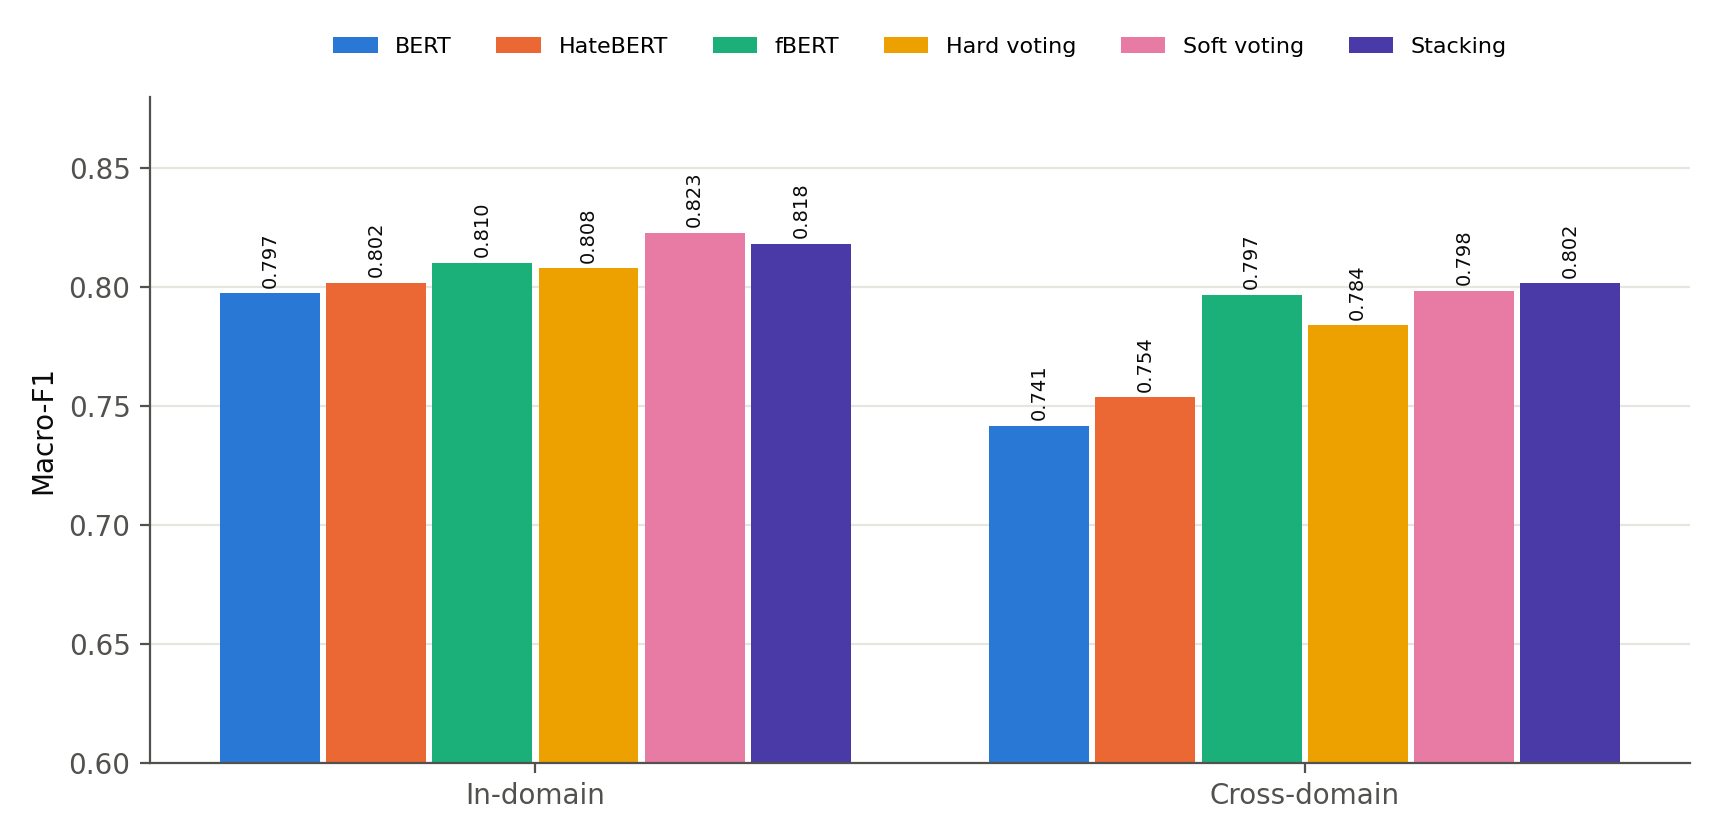
\includegraphics[width=0.92\linewidth]{pics/macro_f1_ensembles.png}
\caption{Macro-F1 of the base models and the three ensembles on the matched pool. The vertical axis starts at 0.60 to make the small differences visible.}
\label{fig:macro}
\end{figure}

In-domain, soft voting is the best system with a macro-F1 of 0.8226, followed by stacking with 0.8180. Both are above fBERT, the best base model at 0.8102. Hard voting lands just below fBERT, at 0.8078.

Cross-domain the order changes a bit. Stacking is best with 0.8016, soft voting reaches 0.7984 and fBERT 0.7966. Hard voting is again below fBERT. So the two probability-based ensembles beat the best single model in both settings, while hard voting does not beat it in either.

Table~\ref{tab:perclass} shows the scores per class. The offensive class is clearly harder for every system, with F1 between 0.61 and 0.74, against 0.86 to 0.90 for the non-offensive class. The per-class scores also show where the gains come from. Stacking and soft voting mainly improve precision on the offensive class. Cross-domain, stacking reaches an offensive precision of 0.7947 against 0.7512 for fBERT, but its offensive recall is a bit lower. It flags fewer tweets, and is right more often when it does.

\subsection{Effect of the extra stacking features}

Stacking with only the three probabilities scores 0.8146 in-domain and 0.7997 cross-domain. The six text features add 0.3 points in-domain and 0.2 points cross-domain. This is a small effect. The meta-model coefficients tell the same story. After standardisation, the fBERT probability has a weight of 1.36 in-domain, while no text feature gets more than 0.31. Cross-domain, the weights are more balanced, with 0.48 for fBERT, 0.32 for BERT and 0.19 for HateBERT. So the meta-model trained on HASOC relies less on fBERT alone.

\subsection{Original block results}
\label{sec:original}

Table~\ref{tab:original} shows the ensembles as first built by each block, before the base models were matched. These use the Assignment 4 models, with a retrained BERT for soft voting.

\begin{table}[H]
\centering
\caption{Macro-F1 of the ensembles as originally built in each block. These use the Assignment 4 base models, so they are not directly comparable with Table~\ref{tab:main}.}
\label{tab:original}
\begin{tabular}{lrr}
\toprule
System & In-domain & Cross-domain \\
\midrule
fBERT, Assignment 4 & 0.8033 & 0.8088 \\
Hard voting, Assignment 4 models & 0.8018 & 0.7863 \\
Soft voting, Assignment 4 models with retrained BERT & 0.8030 & 0.7813 \\
\bottomrule
\end{tabular}
\end{table}

With these base models, neither voting method beats fBERT. One detail looks strange but is correct. The in-domain hard voting result is exactly the same as HateBERT in Assignment 4, down to the confusion matrix. Hard voting disagrees with HateBERT on 38 tweets, but the gains and losses cancel out exactly. The difference with Table~\ref{tab:main} also shows how much the base models matter. The fBERT model from Assignment 4 was unusually strong cross-domain, and the seed check in Assignment 4 gave cross-domain scores between 0.804 and 0.811 for fBERT. The matched pool fBERT scores 0.797, which is within normal training variation.

% ------------------------------------------------------------------
\section{Analysis}
\label{sec:analysis}
% ------------------------------------------------------------------

The analysis focuses on stacking. It is the best system cross-domain, where the qualitative analysis takes place, and it has the smallest cross-domain drop of all ensembles. Soft voting is slightly better in-domain, but the two are not significantly different in either setting, with McNemar p-values of 0.71 in-domain and 0.39 cross-domain.

\subsection{Improvement over the best single model}

Table~\ref{tab:mcnemar} compares each ensemble with fBERT, tweet by tweet.

\begin{table}[H]
\centering
\caption{Exact McNemar tests of each ensemble against fBERT on the matched pool. The middle columns count the tweets that only one of the two systems gets right.}
\label{tab:mcnemar}
\begin{tabular}{llrrr}
\toprule
Setting & Ensemble & Only ensemble right & Only fBERT right & p-value \\
\midrule
In-domain    & Hard voting & 10 & 12 & 0.832 \\
In-domain    & Soft voting & 21 & 12 & 0.163 \\
In-domain    & Stacking    & 6  & 0  & 0.031 \\
\midrule
Cross-domain & Hard voting & 21 & 28 & 0.392 \\
Cross-domain & Soft voting & 24 & 21 & 0.766 \\
Cross-domain & Stacking    & 23 & 16 & 0.337 \\
\bottomrule
\end{tabular}
\end{table}

In-domain, stacking improves on fBERT by 0.8 macro-F1 points. The gain is small but consistent. Stacking fixes 6 fBERT errors and does not introduce a single new one, so the improvement is significant with p = 0.03. Soft voting gains more on paper, 1.2 points, but it fixes 21 errors and breaks 12, which is not significant.

Cross-domain, the picture is less clear. Stacking still wins by 0.5 points, but it changes more predictions, fixing 23 fBERT errors and creating 16 new ones. This is not significant. So the answer to the first question of the assignment is yes in-domain and only weakly cross-domain.

The cross-domain drop is clearly smaller for the ensembles than for most single models. Stacking loses 1.65 macro-F1 points from in-domain to cross-domain, a relative drop of 2.0 percent. Soft and hard voting both lose about 2.4 points. BERT and HateBERT lose 5.6 and 4.8 points. Only fBERT, with a drop of 1.4 points, is as stable as stacking. As discussed in Assignment 4, this comes from its pre-training on SOLID, which uses the OLID labelling scheme.

\subsection{Why the gains are small}

\subsubsection{Comparable results}

The base models are close to each other in-domain, between 0.797 and 0.810 macro-F1. Cross-domain they are not. fBERT scores 0.797, while BERT and HateBERT stay at 0.742 and 0.754. This explains why hard voting falls behind fBERT cross-domain. Two weaker models can outvote the strongest one, and they often do. Soft voting suffers less from this, since a confident fBERT probability can still win. Stacking avoids the problem best, because it learns from the training data how much to trust each model.

\subsubsection{Correlation between the base models}

Table~\ref{tab:pearson} and Figure~\ref{fig:pearson} show the Pearson correlations between the base models.

\begin{table}[H]
\centering
\caption{Pearson correlations between the base models on the OLID test set, for predicted probabilities, predicted labels and error indicators. The last column is the share of tweets where both models predict the same label.}
\label{tab:pearson}
\begin{tabular}{llrrrr}
\toprule
Setting & Pair & r probabilities & r labels & r errors & Same label \\
\midrule
In-domain    & BERT and HateBERT  & 0.831 & 0.726 & 0.594 & 0.891 \\
In-domain    & BERT and fBERT     & 0.892 & 0.814 & 0.723 & 0.927 \\
In-domain    & HateBERT and fBERT & 0.870 & 0.781 & 0.668 & 0.913 \\
\midrule
Cross-domain & BERT and HateBERT  & 0.765 & 0.625 & 0.549 & 0.858 \\
Cross-domain & BERT and fBERT     & 0.812 & 0.682 & 0.612 & 0.886 \\
Cross-domain & HateBERT and fBERT & 0.772 & 0.631 & 0.519 & 0.858 \\
\bottomrule
\end{tabular}
\end{table}

\begin{figure}[H]
\centering
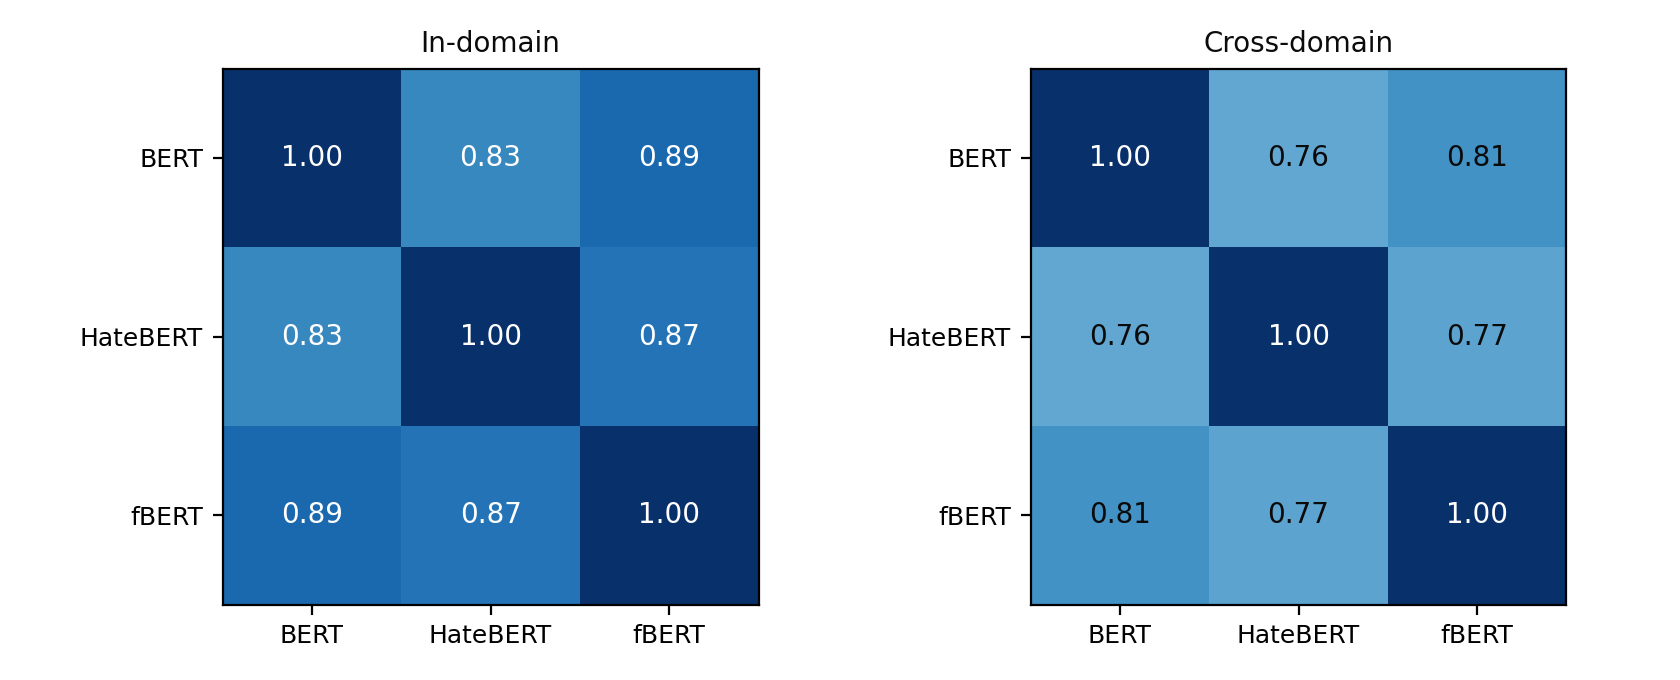
\includegraphics[width=0.8\linewidth]{pics/pearson_probabilities.png}
\caption{Pearson correlation of the predicted offensive probabilities of the base models, in-domain on the left and cross-domain on the right.}
\label{fig:pearson}
\end{figure}

The predictions are far from uncorrelated. The probabilities correlate between 0.76 and 0.89, and even the errors correlate between 0.52 and 0.72. The three models agree on the label of 744 tweets in-domain and 689 cross-domain, out of 860. In each setting there are 79 tweets on which all three are wrong, and no ensemble of these models can fix those.

This was expected. The models share the same fine-tuning data, and all three start from the same uncased BERT base weights and tokenizer. HateBERT and fBERT only differ from BERT in their extra pre-training. Following \citet{kuncheva2003measures}, low diversity means little room for an ensemble to improve. The correlations are lower cross-domain, so the models disagree more there. The ensembles do not turn this extra disagreement into a larger gain, though. Cross-domain, the models disagree on 171 tweets, and on these fBERT is right 67 percent of the time against 47 to 49 percent for BERT and HateBERT. In-domain the gap is much smaller, 56 percent against 48 to 50 percent. So cross-domain, following the majority is often the wrong choice, and only a method that learns to trust fBERT more can profit.

\subsection{Quantitative error analysis}

Figure~\ref{fig:cm} shows the confusion matrices of stacking and Table~\ref{tab:errors} breaks down its errors.

\begin{figure}[H]
\centering
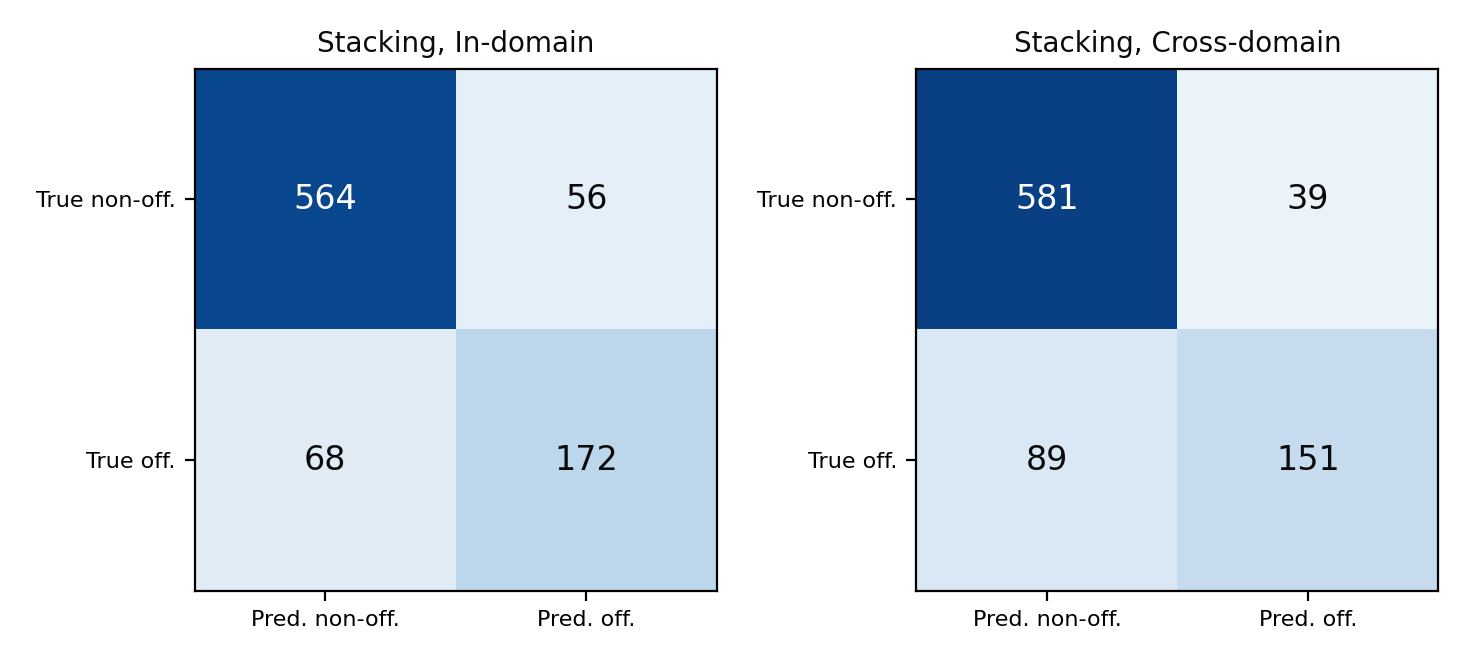
\includegraphics[width=0.78\linewidth]{pics/confusion_stacking.png}
\caption{Confusion matrices of stacking. Rows are gold labels and columns are predictions.}
\label{fig:cm}
\end{figure}

\begin{table}[H]
\centering
\caption{Errors of stacking in both settings. The false positive rate is computed over the 620 non-offensive tweets, the false negative rate over the 240 offensive tweets. The last rows give the share of offensive tweets that are missed, split by whether the tweet contains a swear word.}
\label{tab:errors}
\begin{tabular}{lrr}
\toprule
 & In-domain & Cross-domain \\
\midrule
False positives & 56 & 39 \\
False negatives & 68 & 89 \\
False positive rate & 9.0\% & 6.3\% \\
False negative rate & 28.3\% & 37.1\% \\
\midrule
Error rate, tweets of 0 to 15 words & 14.2\% & 12.4\% \\
Error rate, tweets of 16 to 30 words & 13.8\% & 16.4\% \\
Error rate, tweets of more than 30 words & 15.4\% & 15.7\% \\
\midrule
Missed, offensive tweets with a swear word, 88 tweets & 0.0\% & 5.7\% \\
Missed, offensive tweets without a swear word, 152 tweets & 44.7\% & 55.3\% \\
\bottomrule
\end{tabular}
\end{table}

The type of error changes between the settings. In-domain, the errors are split fairly evenly, with 56 false positives and 68 false negatives. Cross-domain, stacking becomes more careful. False positives drop to 39, but false negatives rise to 89, so more than a third of the offensive tweets are missed. This is the opposite of the Logistic Regression baseline in Assignment 4, which flagged too much when trained on HASOC. The transformer ensemble has learned the stricter HASOC idea of offensive, where swearing alone is not enough.

Message length has little effect. The error rate stays between 12 and 17 percent for all length groups in both settings. Swear words matter much more. Stacking catches every offensive tweet with a swear word in-domain and almost all of them cross-domain. Without a swear word, it misses 45 percent of the offensive tweets in-domain and 55 percent cross-domain. So the main difficulty is offence without explicit words, which matches earlier work on implicit abuse \citep{caselli2020feel}.

\subsection{Qualitative error analysis}

All 128 cross-domain errors of stacking were read and given one main category. Figure~\ref{fig:categories} shows the counts and Table~\ref{tab:categories} gives an example of each category. The categories are based on \citet{vanaken2018challenges}, who describe errors like toxicity without swear words, sarcasm, rhetorical questions and doubtful labels. The hashtag category was added because hashtags are so common in this data.

\begin{figure}[H]
\centering
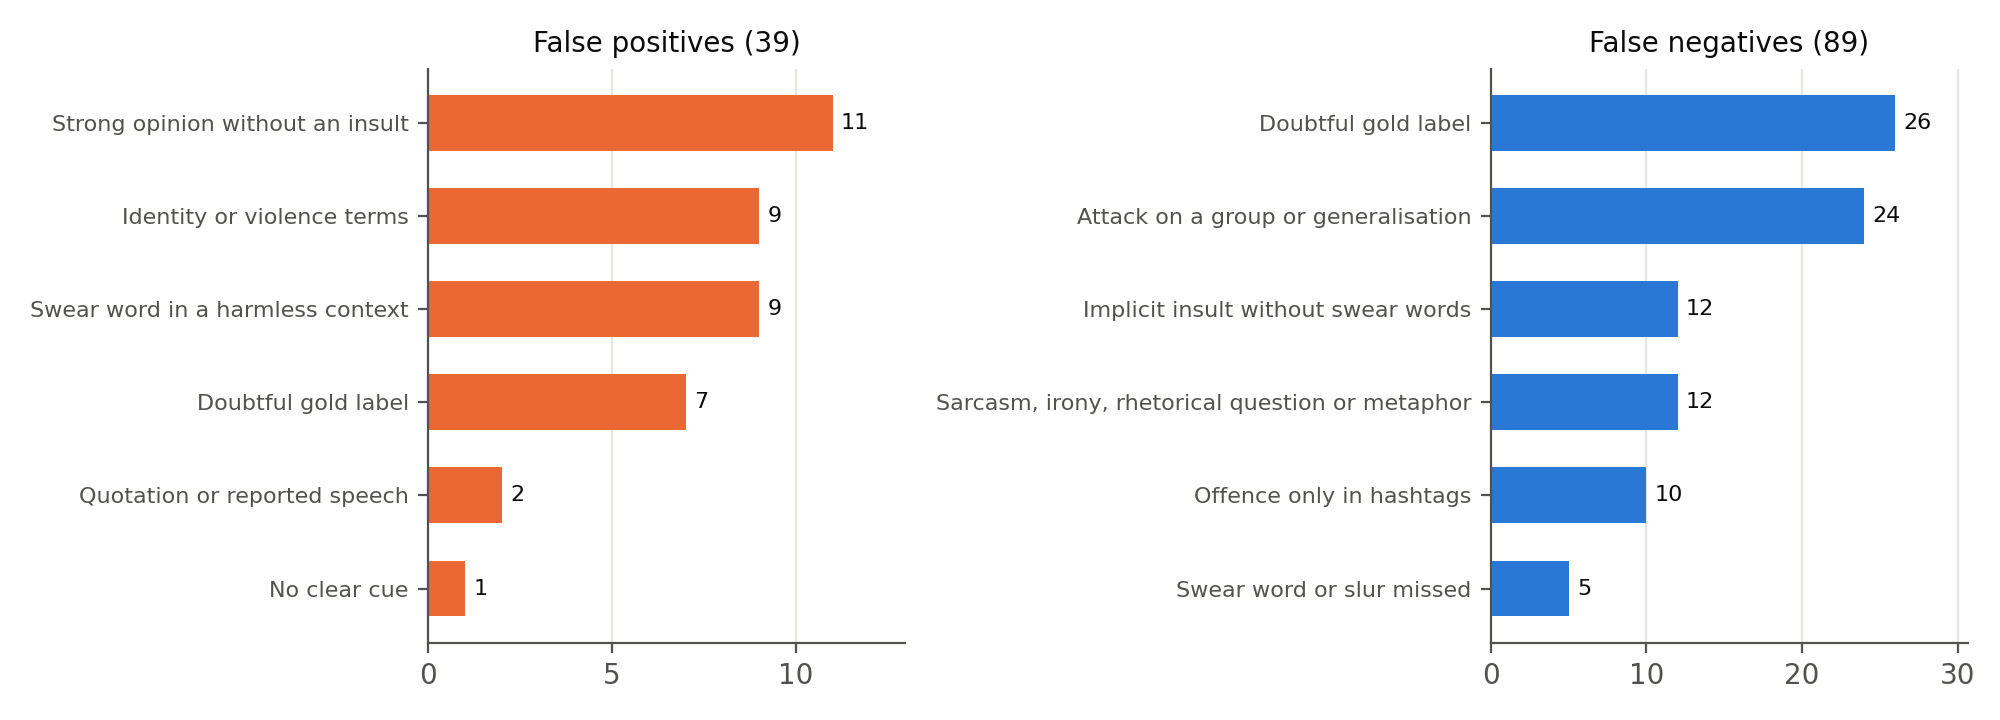
\includegraphics[width=\linewidth]{pics/error_categories_cross_domain.png}
\caption{Main error categories of all cross-domain stacking errors. Each error has exactly one category.}
\label{fig:categories}
\end{figure}

\begin{table}[H]
\centering
\caption{Error categories with an example from the OLID test set. Hashtag signs are left out. FP is a false positive, FN a false negative.}
\label{tab:categories}
\small
\begin{tabular}{L{0.85cm}L{3.9cm}rL{8.1cm}}
\toprule
Type & Category & n & Example \\
\midrule
FP & Strong opinion without an insult & 11 & ChequersPlan What an absolute farce Brexit is. The conservatives have no idea at all and May is now totally discredited. \\
FP & Swear word in a harmless context & 9 & An American Tail really is one of the most underrated animations ever ever ever. Fuck I cried in this scene \\
FP & Identity or violence terms & 9 & AafiaSiddiqui is a convicted terrorist but she is widely hailed as the Daughter of Pakistan. \\
FP & Doubtful gold label & 7 & @USER @USER @USER She is just nasty \\
FP & Quotation or other & 3 & they would have dug up an 8th grade picture of him wearing a hoodie and talk about what a thug he is \\
\midrule
FN & Doubtful gold label & 26 & AmazonPets Etta can be tricky to photograph because of her colouring, but she is BEAUTIFUL and she knows it. \\
FN & Attack on a group or generalisation & 24 & Liberals always up to dirty tricks to get their way. \\
FN & Implicit insult without swear words & 12 & SerenaWilliams is so full of herself, she is just as painful to watch as to listen to \\
FN & Sarcasm, irony, rhetorical question or metaphor & 12 & Who can possibly stand to watch so many liberals in one place at one time. \\
FN & Offence only in hashtags & 10 & DespicableDems lie again about rifles. \\
FN & Swear word or slur missed & 5 & In just 8 short years the @USER have completely fucked the UK \\
\bottomrule
\end{tabular}
\end{table}

\subsubsection{False negatives}

Most missed offensive tweets do not look offensive on the surface. The biggest real category is attacks on a whole group, with 24 cases. Almost all of these target a political group, like liberals, Democrats, antifa or conservatives, with claims such as Liberals always up to dirty tricks to get their way. A few target a religion or a country instead, like a tweet saying that Islam hates every non-Muslim. These tweets contain no swear words and use the same political vocabulary as many harmless OLID tweets. HASOC is also full of political posts about Trump, many of them labelled non-offensive, so a model trained on it learns that strong political statements are normal.

Implicit insults and sarcasm come next, with 12 cases each. Calling someone so full of herself or nothing more than a racebaiter is clearly insulting, but needs no explicit word. Sarcastic tweets, like Who can possibly stand to watch so many liberals in one place at one time, or the remark that a real leader falls into a van like a sack of potatoes, are even harder, because their literal meaning is not offensive. Comparisons work the same way, as in Conservatives just like old garbage bags blowing in the wind.

A smaller but interesting group of 10 tweets carries the offence only in hashtags, like DespicableDems or FemiNazis. The tokenizer splits such hashtags into pieces that no longer look like words. DespicableDems becomes des, pic, able, de and ms, so the model never sees the word despicable. Even a swear word can disappear this way, as dumberthandogshit ends up as dumb, ert, hand, og, shi and t. Only 5 false negatives contain a swear word or slur that was missed. One of them says the government completely fucked the UK, which HASOC would probably label as non-offensive, since it criticises a government and does not insult a person.

\subsubsection{False positives}

The false positives are more varied. In 11 cases the tweet gives a strong political opinion without insulting anyone, like calling Brexit an absolute farce or asking voters to DUMP Susan Collins. Another 9 use swear words in a harmless way, for example Fuck I cried in this scene about a children's film, or Damn about a wrestling match. These look offensive to a model that relies on explicit words, even though HASOC taught it that swearing is not enough. Another 9 mention terrorism, fascism, murder or religious groups in a neutral or even supportive way, like a tweet remembering an antifa rapper who was stabbed to death. False positives like these are a known problem in cross-domain hate speech detection \citep{markov2021improving}.

\subsubsection{Doubtful labels}

Not every error is the model's fault. For 26 false negatives and 7 false positives, the gold label itself is hard to defend. Tweets about a pet, a TV series, government debt or a news report on a protest, and even the single test tweet that only reads NAME with a question mark, are labelled offensive. On the other side, She is just nasty is labelled non-offensive. Together these make up a quarter of all cross-domain errors. \citet{vanaken2018challenges} found the same problem in their data. It means the real performance of the models is somewhat higher than the scores suggest, and that some remaining errors cannot be fixed by better models.

\subsection{How the errors can be reduced}

Each type of error calls for a different fix.

\textbf{Group attacks and implicit insults.} The models need examples where groups are targeted without swear words. OLID has a third level that labels whether an offence targets an individual or a group \citep{zampieri2019olid}. Training on this level, or adding a target detector as a stacking feature, could help the model notice when a whole group is being attacked. Also, adding OLID or SOLID data to the HASOC training set would give the model the OLID view of political attacks.

\textbf{Sarcasm and metaphors.} A separate sarcasm or irony classifier could provide another stacking feature. A large language model prompted with the full tweet could also be added as a fourth base model. It works in a very different way from the BERT models, so its errors would probably be less correlated with theirs.

\textbf{Offence in hashtags.} Hashtags can be split into words before tokenization, so DespicableDems becomes despicable dems. This is cheap and only changes the input.

\textbf{False positives from swear words and identity terms.} A swear word count could be added as a stacking feature, so the meta-model can learn when swearing matters and when it does not. For identity and violence terms, the training data can be extended with neutral sentences that mention these terms, so the model stops treating them as offensive on their own.

\textbf{Doubtful labels.} These can only be fixed in the data, by relabelling unclear cases or by using labels from several annotators instead of one.

% ------------------------------------------------------------------
\section{Discussion and conclusion}
\label{sec:conclusion}
% ------------------------------------------------------------------

\subsection{Summary of findings}

Combining the three BERT models helps, but only a little. On a shared set of base models, soft voting and stacking both beat the best single model, by 1.2 and 0.8 macro-F1 points in-domain and by 0.2 and 0.5 points cross-domain. Only the in-domain gain of stacking is significant. Hard voting does not beat fBERT in either setting. Stacking keeps the cross-domain drop small, at 1.65 points, compared with about 5 points for BERT and HateBERT. The hypothesis is therefore confirmed. The gains are small because the base models are highly correlated, with error correlations between 0.52 and 0.72, and because all three are wrong on the same 79 tweets.

The error analysis shows that the main remaining challenge is offence without explicit words. Cross-domain, stacking misses 55 percent of the offensive tweets without a swear word. Most of these are attacks on political groups, and many others are implicit insults or sarcastic remarks. About a quarter of all errors involve gold labels that are hard to defend.

\subsection{Reflection}

The biggest lesson from this assignment was about the comparison itself. The first versions of hard and soft voting were built on slightly different base models, and the differences between those runs were as large as the differences between the ensemble strategies. A different BERT run changed 132 cross-domain predictions. Without the matched pool, the conclusion would have been that no ensemble beats fBERT. With it, the probability-based ensembles do. So with small gains like these, the base models have to be held fixed, and seed variation has to be kept in mind. The fBERT model from Assignment 4 scored 0.809 cross-domain, higher than any ensemble here.

Stacking was also by far the most expensive method, with eighteen extra training runs, for a gain that is not significant cross-domain. Soft voting reached almost the same scores with no training at all. In practice, soft voting is a strong and cheap default, and stacking is mainly worth it when the base models differ a lot in quality, as they do cross-domain.

\subsection{Future work}

The most promising step is more diversity among the base models. The ensemble could include a model of a different kind, such as a large language model used in a zero-shot setting, or BERT models fine-tuned on other offensive language datasets. Another option is to give stacking features that target the errors found here, like a swear word count or a sarcasm score, and to split hashtags into words before tokenization. Finally, all experiments should be repeated over several seeds, since the differences between the systems are of the same size as the variation between training runs.

\bibliographystyle{plainnat}
\bibliography{references}

\appendix

% ------------------------------------------------------------------
\section{Division of work}
% ------------------------------------------------------------------

The work was split so that each member kept working with the model they used in Assignment 4.

\textbf{Ines Casado Vela} prepared the common Assignment 5 notebook with the Assignment 4 predictions of the three transformer models, checked these predictions, and built and evaluated hard majority voting in both settings. She also wrote the first version of the hard voting section.

\textbf{Helian X. Liu} retrained BERT to obtain prediction probabilities, built and evaluated soft majority voting in both settings, and wrote the first version of the soft voting section.

\textbf{Martin Ranea Marina} exported the HateBERT probabilities, trained the out-of-fold models for stacking, built and evaluated the stacking ensemble with the extra text features, and recomputed both voting methods on the matched pool. He also wrote the first version of the stacking section.

\textbf{Pablos Tselioudis Garmendia} provided the fBERT probabilities from Assignment 4, computed the Pearson correlations and the significance tests, carried out the quantitative error analysis and the manual analysis of all 128 cross-domain errors, and did the final integration, including the final notebook and the writing of this report.

% ------------------------------------------------------------------
\section{Code and files}
% ------------------------------------------------------------------

The notebook and all files are available in this GitHub repository.

\begin{center}
\url{https://github.com/PablosTsel/subjectivity-mining-a5-group9}
\end{center}

The repository contains the final notebook, A5-notebook-Group9-FINAL.ipynb, which has the code and outputs of all four parts, and the three dataset files. Each part has its own folder with its predictions, probabilities and scores. The stacking folder also holds the training scripts, the out-of-fold features and the run records of every trained model. The analysis folder holds the error annotations of all 128 cross-domain errors, the correlation tables and the figures used in this report.

\end{document}
